\section{Main Window}
    For a better understanding of further comments and instructions, lets define five major areas of the main window.

   \begin{figure}[h]
        \centering
        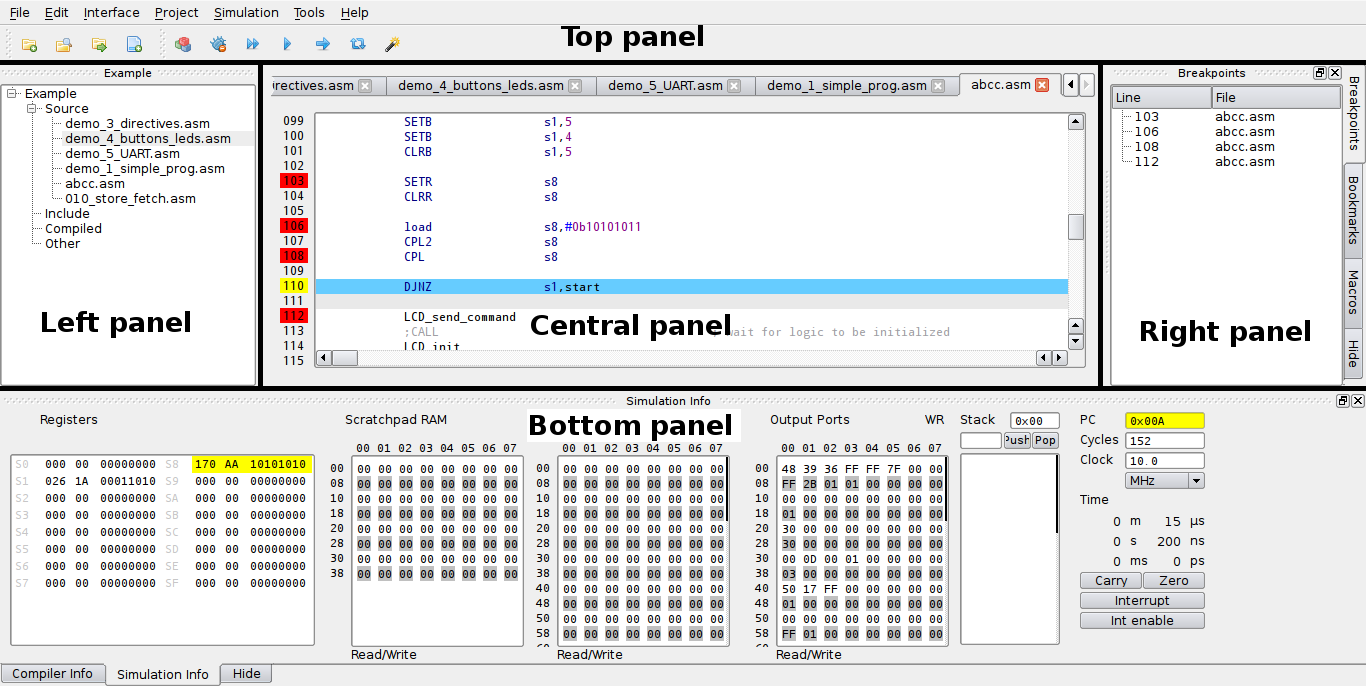
\includegraphics[width=\textwidth]{img/Main_window.png}
        \caption{Layout of the main window}
    \end{figure}

    \clearpage
    \subsection{Left and right panel}
        \begin{table}[h!]
            \centering
            \begin{tabular}{cc}
                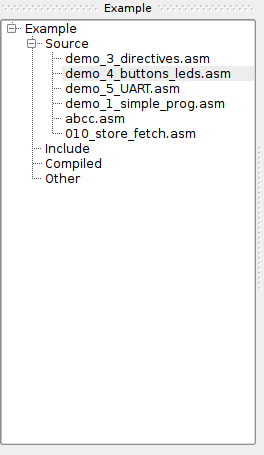
\includegraphics[width=.3\textwidth]{img/left_panel.png}
                    &
                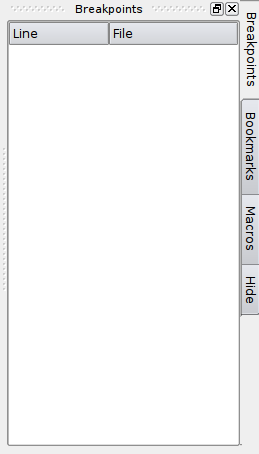
\includegraphics[width=.3\textwidth]{img/right_panel.png}
                    \\
                Left panel & Right panel
            \end{tabular}
        \end{table}

        \subsubsection{Left panel}
            \index{Left panel}
            Left panel displays files in your project tree. Also it allows to perform various actions via context menus (right click), like: configure project, close project, open file, close file, remove file from this list, or set some file as the project's main source file, etc.

        \subsubsection{Right panel}
            \index{Right panel}
            Right panel contains lists of breakpoints, bookmarks, and macros defined in your source code. From these lists you can easily navigate to the corresponding line in your source code just by clicking on an item. List of macros might sometimes need to refresh which can be achieved by [Right~Click] -> [Refresh].

            \begin{table}[h!]
                \begin{tabular}{ccc}
                    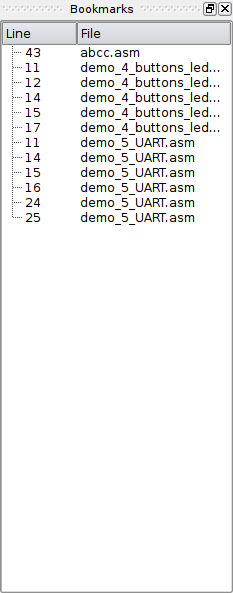
\includegraphics[width=.3\textwidth]{img/listbookmarks.png}
                        &
                    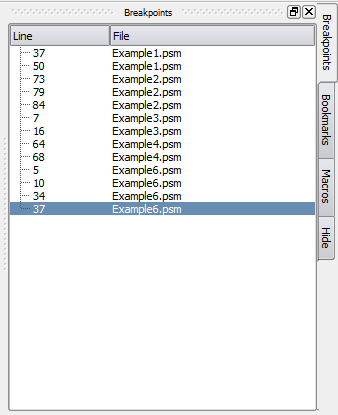
\includegraphics[width=.3\textwidth]{img/listbreakpoints.png}
                        &
                    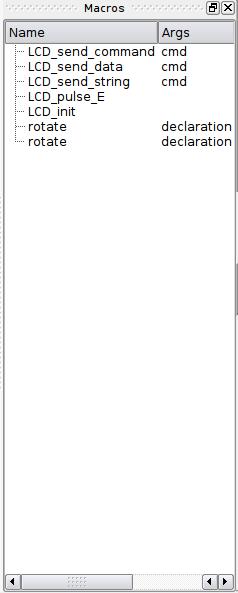
\includegraphics[width=.3\textwidth]{img/listmacros.png}
                    \\ Bookmarks & Breakpoints & Macros
                \end{tabular}
            \end{table}

    \subsection{Central panel}
        Central panel contains the main text editor with syntax highlight for writing a source code. In the editor you can also easily add breakpoints and bookmarks just by clicking on desired line number by left or right mouse button, each invokes different action.

    \subsection{Top panel}
        \index{Toolbar}
        Top panel contains main menu and the toolbar, both can be used to invoke various actions which are described alter in this documentation.

        \begin{figure}[h!]
            \centering
            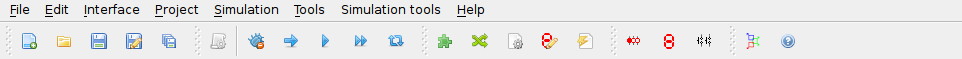
\includegraphics[width=.9\textwidth]{img/top_panel.png}
            \caption{Top panel}
        \end{figure}

    \subsection{Bottom panel}
        Bottom panel consists of simulator main panel and compiler messages.

        In simulator main panel you can see status of internal registers, scratch-pad ram, input and output ports, call
        stack, program counter, elapsed time, elapsed machine cycles, processor clock, and internal flags: carry, zero, interrupt, and interrupt enable. Most of these values can be edited during processor simulation.

        In compiler messages panel you can see textual output from the assembler, like warnings and other messages.

        \begin{figure}[h!]
            \centering
            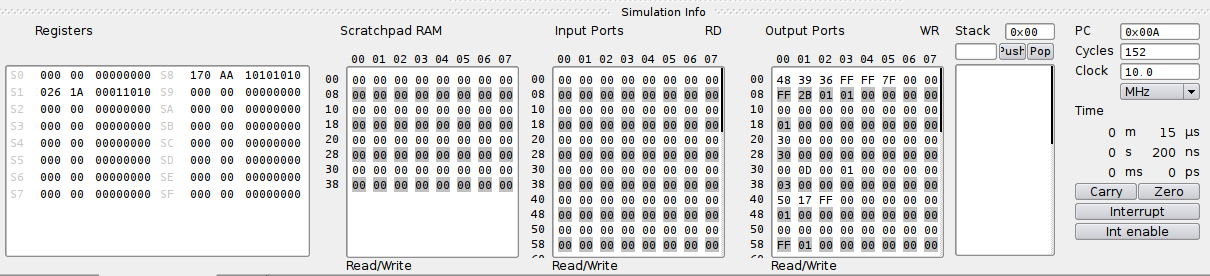
\includegraphics[width=.9\textwidth]{img/bottom_panel.png}
            \caption{Bottom panel}
        \end{figure}

    \clearpage
    \subsection{Exit \& Restoration}
        \subsubsection{Session Restoration}
            When the main window is closed on user request, the MDS automatically saves the current session and restores it when run again. The session includes list of opened projects. When you run MDS, the projects and their files from the last session are automatically reopened as they were last time when you closed the MDS window.

        \subsubsection{Exit Dialog}
            \begin{wrapfigure}{r}{0pt}
                \centering
                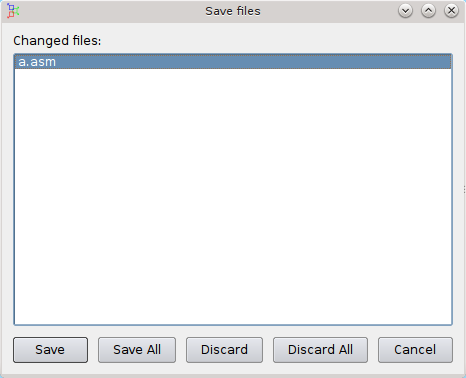
\includegraphics[width=130pt]{img/exit_dialog.png}
                \caption{Exit Dialog}
            \end{wrapfigure}

            When closing the main window, MDS automatically checks if all files which you have been working on have been saved on the disk; and if some of them have not, it displays a dialog (Exit Dialog) asking you which files you want to save and which not. But be aware that this function cannot possibly handle (unlikely) possibility of program crash, we recommend that you save your files regularly to prevent accidental data loss.

            \begin{description}
                \item[Button Save:] Saves the selected file; and if there is only one file left, exits the IDE.
                \item[Button Save All:] Saves all files and exits the IDE.
                \item[Button Discard:] Discards recent changes in the selected file; if there is only one file left, exits the IDE.
                \item[Button Discard All:] Discards recent changes in all files and exits the IDE.
                \item[Button Cancel:] Closes the dialog and returns to the IDE, the main window will remain opened.
            \end{description}

    \subsection{Main menu actions}
        \begin{description}
            \item[File / New File] Create a new file in your current project.
            \item[File / New Untracked File] Create a new file outside your current project.
            \item[File / Open File] Open an existing file and add it to your current project.
            \item[File / Open Recent] Keeps track of recently opened files and allows to easily reopen them.
            \item[File / Save File] Save the current file in the current project.
            \item[File / Save As] Save the current file in the current project under a different name.
            \item[File / Save All] Save all opened files in all opened projects.
            \item[File / Exit] Exit the MDS environment.

            \item[Edit / Undo] Undo the last editing action in the code editor.
            \item[Edit / Redo] Revert the last undo action.
            \item[Edit / Cut] Cut the selected text in the code editor and copy it into clipboard.
            \item[Edit / Copy] Copy the selected text into clipboard.
            \item[Edit / Paste] Paste the clipboard content into the code editor.
            \item[Edit / Select All] Select all text in the code editor.
            \item[Edit / Deselect] Deselect the selected text in the code editor.

            \item[Interface / Configure] Open user interface configuration dialog.

            \item[Project / New Project] Open wizard for creating new projects.
            \item[Project / Open Project] Open and existing MDS project.
            \item[Project / Open Recent] Keeps track of recently opened MDS projects and allows to easily reopen them.
            \item[Project / Save Project] Save all opened files in the current project.
            \item[Project / Close Project] Close the current project.
            \item[Project / Compile] Run compiler on your current file or the main file in your current project.
            \item[Project / Save Project Config] Save the project configuration (compiler settings, etc., not the source files them selfs).
            \item[Project / Configure] Open project configuration dialog.

            \item[Simulation / Start Simulation] Start processor simulator with machine code generated from the current file or the main file.
            \item[Simulation / Run] Run the program loaded in the simulator.
            \item[Simulation / Animate] Animate the program loaded in the simulator.
            \item[Simulation / Step] Execute one instruction cycle in the simulator.
            \item[Simulation / Reset] Reset simulator.
            \item[Simulation / Unhighlight] Remove highlight for recently changed values in the simulator GUI components.
            \item[Simulation / Breakpoint] Set breakpoint for the current line in the current file.
            \item[Simulation / Disable Breakpoints] Disable simulator breakpoints generally.
            \item[Simulation / Enable Breakpoints] (Re-)Enable simulator breakpoints generally.

            \item[Tools / Disassembler] Open disassembler dialog.
            \item[Tools / Assembler translator] Open Assembler Translator dialog.
            \item[Tools / Data File Converter] Open Data File Converted utility.
            \item[Tools / Radix Converter] Open Radix Converter utility.
            \item[Tools / 8 Segment Editor] Open single digit LED display editor.
            \item[Tools / Loop Generator] Open Loop Generator utility.

            \item[Simulation Tools / LED Panel] Open simple LED panel simulator.
            \item[Simulation Tools / 7 Segment Display] Open simple LED display simulator.
            \item[Simulation Tools / Switch Panel] Open simple switch panel simulator.

            \item[Help / About] Displays basic information about your MDS version.
            \item[Help / User Manual] Open user manual, this document.
            \item[Help / Open Tutorial Project] Open the Tutorial Project, each user should read the tutorial before using this IDE.
            \item[Help / Welcome Dialog] Reopen the welcome dialog, you have already seen the welcome dialog when you first started the MDS.
            \item[Help / About Qt] Display basic information about the Nokia Qt framework.
            \item[Help / License] Display detailed information about the terms of license for this product.
        \end{description}

        \subsubsection{Action shortcuts}
            \index{Main window shortcuts}
            These are the key shortcuts for the main windows, code editor shortcuts will be shown later in this manual.

            \begin{table}[h!]
                \centering
                \fontsize{8pt}{9pt}
                {
                    \begin{tabular}{|ll|ll|}
                        \hline
                        \textbf{Shortcut}               & \textbf{Description}          &
                        \textbf{Shortcut}               & \textbf{Description}          \\\hline
                        \texttt{Ctrl + N}               & New file                      &
                        \texttt{Ctrl + O}               & Open file                     \\
                        \texttt{Ctrl + S}               & Save file                     &
                        \texttt{Ctrl + W}               & Close file                    \\
                        \texttt{Ctrl + Shift + S}       & Save As                       &
                        \texttt{Ctrl + L}               & Save All                      \\
                        \texttt{F5}                     & Compile                       &
                        \texttt{F6}                     & Start simulator               \\
                        \texttt{F7}                     & Simulator: Run                &
                        \texttt{F8}                     & Simulator: Animate            \\
                        \texttt{F9}                     & Simulator: Step               &
                        \texttt{F10}                    & Simulator: Reset              \\
                        \hline
                    \end{tabular}
                }
                \caption{Default key shortcuts for the Main Window.}
            \end{table}

\clearpage
\section{Code Editor}
    \index{Code editor}
    Code editor is optimized for writing source code for your applications, it behaves as is generally expected from a code editor. The editor has two different modes of operations:

    \begin{enumerate}
        \item Editing mode: for editing your files, this mode is for reading and writing/editing.
        \item Simulation mode: for displaying progress of the program simulation, in this mode the displayed code is for reading only.
    \end{enumerate}

    \subsection{Main features}
        \subsubsection{Syntax highlight}
            Syntax highlight is supported only for the PicoBlaze assembly language. Syntax highlighting is automatically activated for files with extension \texttt{.asm} and \texttt{.psm}, otherwise syntax highlight stays inactive.

        \subsubsection{Left panel}
            For easier navigation, the editor's left panel shows line numbers in your code, bookmarks, and breakpoints.

        \subsubsection{Editor status bar}
            Editor status bar displays information about current column and line number.

        \subsubsection{Context menu}
            Context menu pops-up when you right click in the editor or when you press the Menu key (available on some keyboards), it provides means to perform some basic operations like Cut, Copy, Paste, etc.

    \enlargethispage{6\baselineskip}
    \subsection{Key shortcuts}
        \index{Editor shortcuts}
        \begin{table}[h!]
            \centering
            \fontsize{8pt}{9pt}
            {
                \begin{tabular}{|ll|ll|}
                    \hline
                    \textbf{Shortcut}                       & \textbf{Description}          &
                    \textbf{Shortcut}                       & \textbf{Description}          \\\hline
                        \texttt{Ctrl + X}                   & Cut                           &
                        \texttt{Ctrl + C}                   & Copy                          \\
                        \texttt{Ctrl + V}                   & Paste                         &
                        \texttt{Ctrl + Z}                   & Undo                          \\
                        \texttt{Ctrl + Shift + Z}           & Redo                          &
                        \texttt{Ctrl + D}                   & Comment                       \\
                        \texttt{Ctrl + Shift + D}           & Uncomment                     &
                        \texttt{Ctrl + B}                   & Set bookmark                  \\
                        \texttt{Ctrl + Shift + B}           & Set breakpoint                &
                        \texttt{Ctrl + A}                   & Select all                    \\
                        \texttt{Ctrl + Shift + A}           & Deselect                      &
                        \texttt{Ctrl + G}                   & Go to line                    \\
                        \texttt{Ctrl + F}                   & Find                          &
                        \texttt{F3}                         & Find next                     \\
                        \texttt{Shift + F3}                 & Find previous                 &
                        \texttt{Ctrl + R}                   & Replace                       \\
                        \texttt{Ctrl + Up}                  & Scroll one line up            &
                        \texttt{Ctrl + Down}                & Scroll one line down          \\
                        \texttt{Ctrl + Left}                & Move cursor one word left     &
                        \texttt{Ctrl + Right}               & Move cursor one word right    \\
                        \texttt{Ctrl + U}                   & Convert to uppercase          &
                        \texttt{Ctrl + Shift + U}           & Convert to lowercase          \\
                        \texttt{Ctrl + Alt + U}             & Capitalize                    &
                        \texttt{Ctrl + K}                   & Delete line                   \\
                        \texttt{Ctrl + T}                   & Swap characters               &
                        \texttt{Ctrl + H}                   & Select word under cursor      \\
                        \texttt{Ctrl + Shift + Left}        & Select one word to the left   &
                        \texttt{Ctrl + Shift + Right}       & Select one word to the right  \\
                        \texttt{Ctrl + Shift + Up}          & Move line up                  &
                        \texttt{Ctrl + Shift + Down}        & Move line down                \\
                        \texttt{Alt + PageUp}               & Go to previous bookmark       &
                        \texttt{Alt + PageDown}             & Go to next bookmark           \\
                        \hline
                \end{tabular}
            }
            \caption{Default Editor shortcuts.}
        \end{table}

    \clearpage
    \subsection{Breakpoints and bookmarks}
        \index{Breakpoints} \index{Bookmarks}
        \begin{wrapfigure}{r}{0pt}
            \centering
                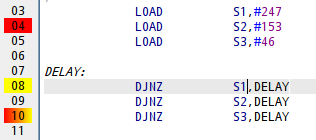
\includegraphics[width=.35\textwidth]{img/breakpoints1.png}
                \caption{Yellow - bookmark, Red - breakpoint, Yellow/Red gradient - both}
        \end{wrapfigure}

        For efficient debugging, our simulator supports breakpoints. Breakpoint is a mark associated with certain location in the program code; when reached, it triggers a temporarily halt in the running simulation. You can use breakpoints to test and debug programs in a manner that the program can be examined in stages delimited by breakpoints. Please be also aware that using breakpoints slows down the simulator (about by 30\% in run mode); if you want to reach the maximum simulation speed, you may temporarily disable (switch off) breakpoints generally in [Main~Menu]~-> [Simulation]~-> [Disable~Breakpoints].

        Another feature is bookmarks; when editing one location in your source code more often, it may be useful to add a bookmark to it so you can quickly get back when you need. Like breakpoints bookmarks are marks in your source code but they are meant solely for quick navigation, they do not affect simulation or compilation in any way.

\section{Project management}
    \index{Project management}
    MDS can organize your files into groups called projects, a project is also bound with its specific configuration which includes:
    \begin{itemize}
        \item Information about which exact processor do you use and in what exact configuration (memory size, etc.).
        \item Compiler settings to be applied: paths to search for included file, which file formats you want to be generated by the assembler, what VHDL template you want to use, etc.
        \item Whether your project comprises of a set of independent files, or if it has one main file and other project files are only included in it using the \texttt{INCLUDE} directive.
    \end{itemize}

    \subsection{Untracked files}
        \index{Untracked files}
        Besides files bound with particular project, you can also open, modify, save, compile, and simulate on files which are not part of your current MDS project. These files, files not bound with a project, we call untracked files, using untracked files has some limitations and under normal circumstances it should be avoided, for instance when you run simulator on an untracked file, note that in that case compiler has to be run first, MDS does not know what processor it should use as target, what is the size of its program memory, whether to generate MEM file or not, etc. All these configuration options can be set for also untracked files but these settings are ultimately lost when you leave the MDS environment, while if you used project, they would be saved. The purpose of project is to provide you better comfort while using this IDE, although in some cases you just do not want to bother with creating a new project just for one file for a few minutes of work, and that is where the untracked files comes handy.

    \clearpage
    \subsection{Project configuration}
        In project configuration window, you can edit project and compiler settings. You can open project configuration
        window by right clicking on project name in the left panel and choosing Configuration, see the pictures below.
        This will open main configuration window with multiple tabs on the left side.

        \subsubsection{Project - Options}
            \begin{itemize}
                \item Project name: Name of your project.
                \item Architecture: Processor architecture used in your project.
                \item Family: Processor family of the selected architecture.
                \item Info panel: Brief description of selected processor.
            \end{itemize}

        \subsubsection{Project - Memory}
            \begin{itemize}
                \item Size options: Memory size.
                \item Interrupt vector: Interrupt vector (size of program memory - 1 is maximum),
                \item HW build: Your HW build constant.
            \end{itemize}
            \begin{table}[h!]
                \begin{tabular}{cc}
                    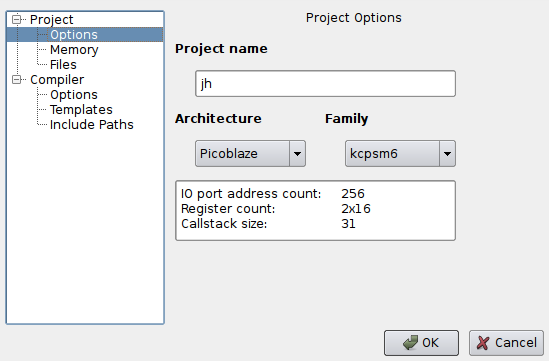
\includegraphics[width=.5\textwidth]{img/config2.png}
                        &
                    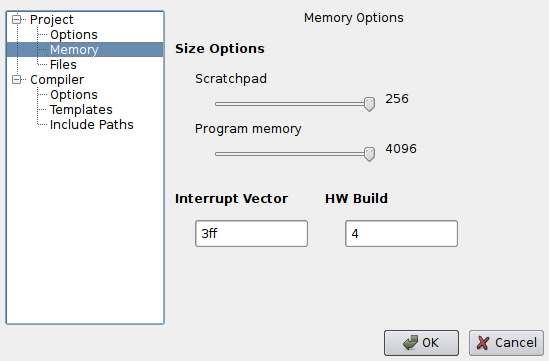
\includegraphics[width=.5\textwidth]{img/config1.png}
                        \\
                    Project - Options & Project - Memory
                \end{tabular}
            \end{table}

        \subsubsection{Project - Files}
            Here is where you can create, add, or remove files from your project, and set set the main file (see below).

        \subsubsection{Compiler - Options}
            \begin{itemize}
                \item
                    \index{Main file}
                    Main file: If you have "Use main file" checked, you can choose which file will always chosen for compilation and simulation instead of the file currently opened in the code editor.
                \item
                    Generate: Select which files should the assembler generate in your project's directory from the given source code.
            \end{itemize}

            \begin{table}[h!]
                \begin{tabular}{cc}
                    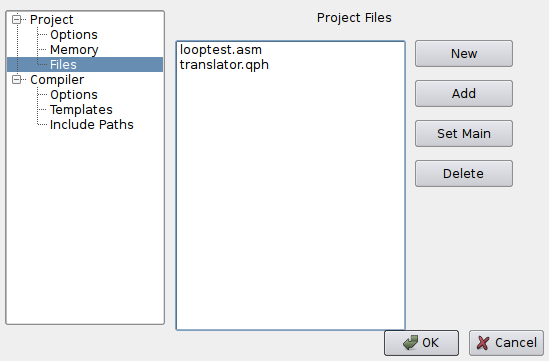
\includegraphics[width=.5\textwidth]{img/config3.png}
                        &
                    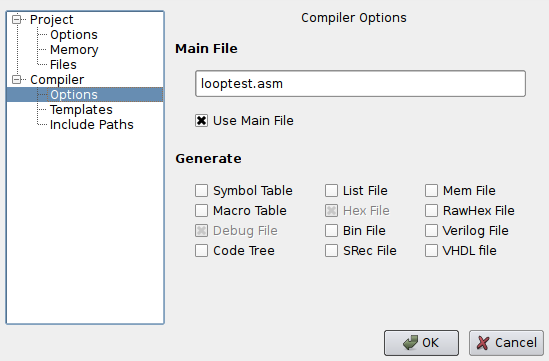
\includegraphics[width=.5\textwidth]{img/config4.png}
                        \\
                    Project - Files & Compiler - Options
                \end{tabular}
            \end{table}

        \subsubsection{Compiler - templates}
            Choose which VHDL or Verilog template will be used by the assembler to generate the HDL code for your
            design, by default MDS uses its own built-in templates.

        \subsubsection{Compiler - include paths}
            Here you can add or edit path, where the compiler will try to find files included in other source code files
            (directive \texttt{INCLUDE}).

            \begin{table}[h!]
                \begin{tabular}{cc}
                    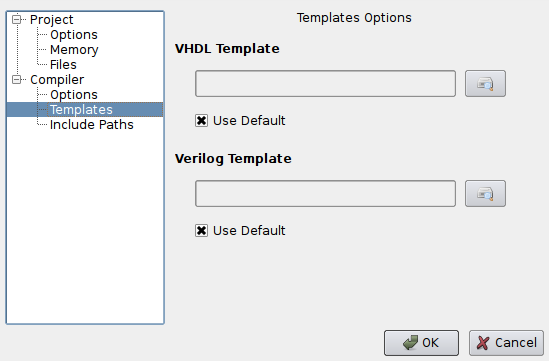
\includegraphics[width=.5\textwidth]{img/config5.png}
                        &
                    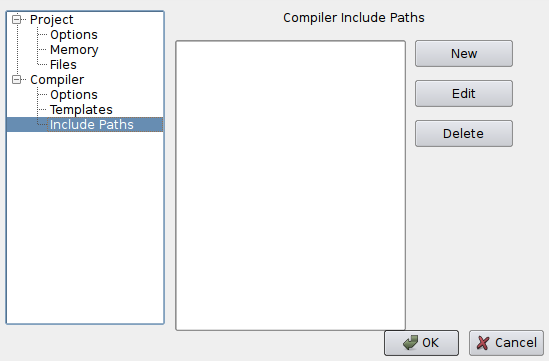
\includegraphics[width=.5\textwidth]{img/config6.png}
                        \\
                    Compiler - Templates & Compiler - Include paths
                \end{tabular}
                \end{table}

\clearpage
\section{UI Configuration}
    In the interface configuration dialog, you can edit appearance and behavior of the IDE. To open the interface configuration dialog, click on [Main~Menu]~-> [Interface]~-> [Configure].

    In the general settings, you can set things like: display the splash screen at start-up, etc. In the code editor settings, you can set tab width, fonts, etc. In simulator settings, you can slightly adjust simulator behavior.

        \begin{table}[h!]
            \begin{tabular}{cc}
                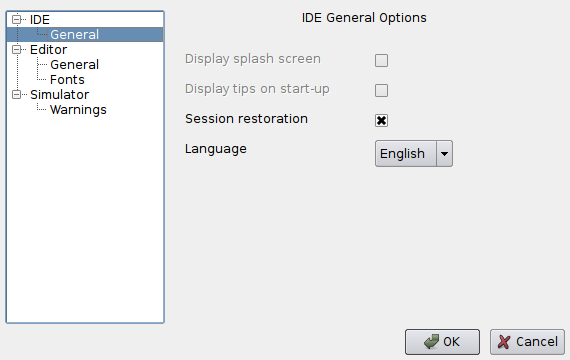
\includegraphics[width=.4\textwidth]{img/interface1.png}
                    &
                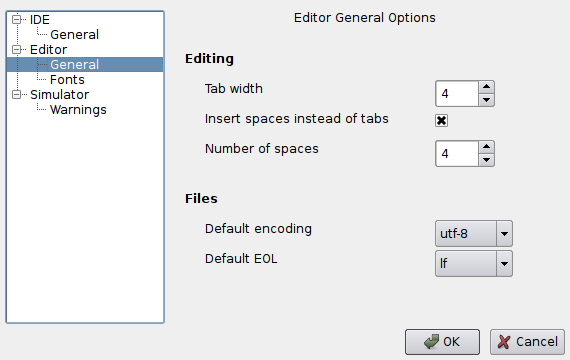
\includegraphics[width=.4\textwidth]{img/interface2.png}
                    \\
                IDE - General & Editor - General
                    \\
                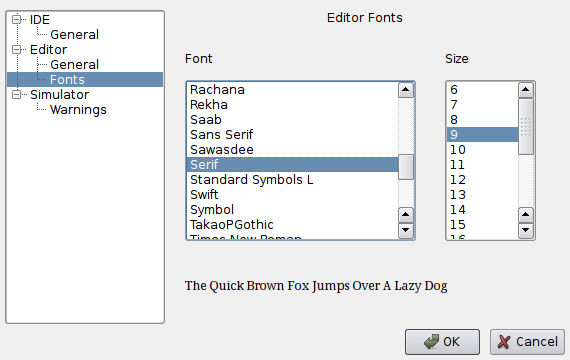
\includegraphics[width=.4\textwidth]{img/interface3.png}
                    &
                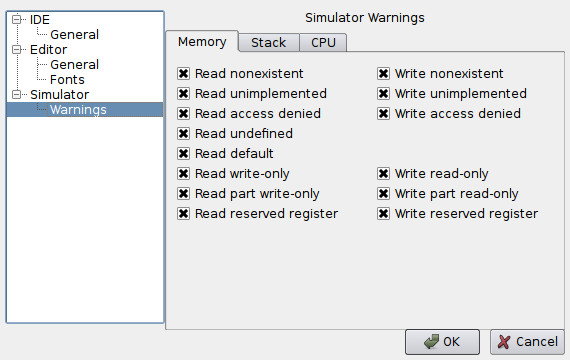
\includegraphics[width=.4\textwidth]{img/interface4.png}
                    \\
                Editor - Fonts & Simulator - Warnings -> Memory
                    \\
                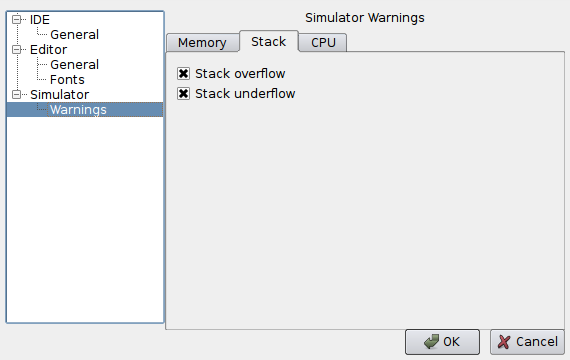
\includegraphics[width=.4\textwidth]{img/interface5.png}
                    &
                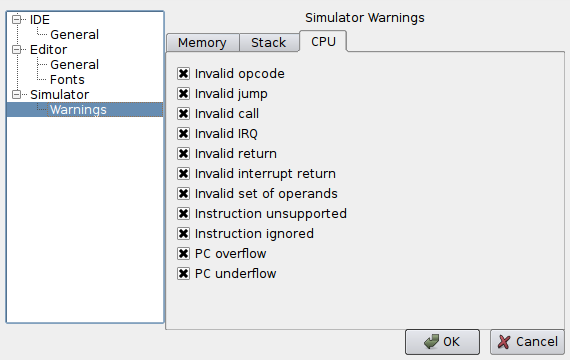
\includegraphics[width=.4\textwidth]{img/interface6.png}
                    \\
                Simulator - Warnings -> Stack & Simulator - Warnings -> CPU
            \end{tabular}
        \end{table}

\clearpage
\section{Tools}
    \subsection{Delay loop generator}
        In many cases, it is useful to have a tool for creating delay loops, it can just save you some time during         development. This tool can generate wait loops using up to six registers as iterators. All you have to do is to enter the desired time of delay or the number of instruction cycles, and clock frequency.

        \begin{description}
            \item[Section Input variable] Choose between time or instruction cycles.
            \item[Section Desired waiting time] Time or number of instruction cycles.
            \item[Section Frequency] Clock frequency.
            \item[Section Register names] Register names to be used in the generated code as iterators.
            \item[Section Generated code] The resulting automatically generated code.
            \item[Instruction] Instruction used in loops.
            \item[Type] Form of delay loop, whether you want it as macro, or plain.
            \item[Upper Case and Comments] Comments: turn on/off automatically added comments; Upper case: use upper case letters.
            \item[Button Copy to clipboard] Copy the generated code into clipboard.
            \item[Button Generate] Generate the code.
        \end{description}

        \enlargethispage{6\baselineskip}
        \begin{figure}[h]
            \centering
            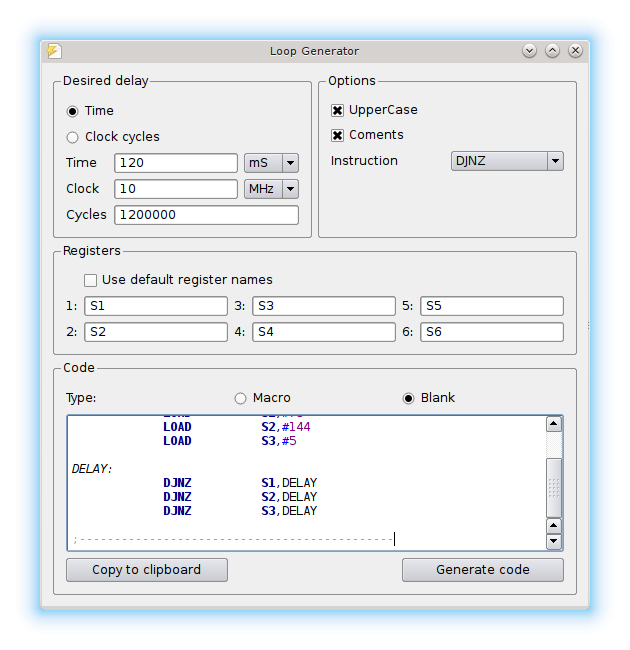
\includegraphics[width=.6\textwidth]{img/loop_gen.png}
            \caption{Delay loop generator}
        \end{figure}

    \clearpage
    \subsection{Disassembler}
        Disassembler is a tool that translates machine language into assembly language. The inverse operation to that of an assembler.

        \begin{description}
            \item[Section File] File you want to disassemble.
            \item[Section Target] Processor architecture
            \item[Family] Processor family of the selected architecture.
            \item[Indentation] Whether you want to indent the generated code with tabs or spaces.
            \item[Tab size] Tab size (measured in number of spaces).
            \item[Radix] Radix for numeric literals in the resulting code: binary, octal, decimal, or hexadecimal.
            \item[Line break] CRLF (Windows), LF (Linux), or CR (Mac)
            \item[Case] Use uppercase or lowercase characters.
            \item[Generate symbols] Which types of values should be defined as symbols in resulting code.
        \end{description}

        \begin{figure}[h]
            \centering
            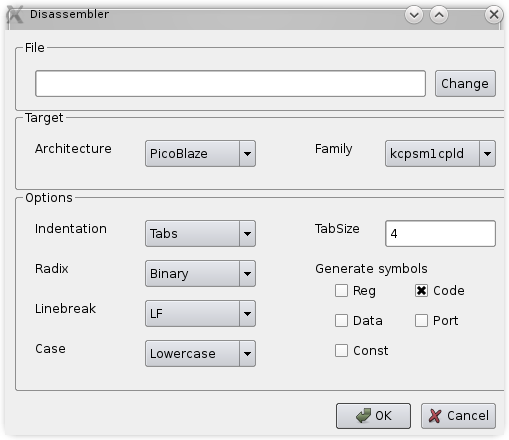
\includegraphics[width=.5\textwidth]{img/disassembler_window.png}
            \caption{Disassembler}
        \end{figure}

\clearpage
    \subsection{Assembler translator}
        With this tool, you can translate your previously written assembler code in different syntax that MDS uses. You can select one of three choices for input file syntax: Xilinx, Mediatronix, and OpenPicIde. Input code has to be without errors.

        \begin{description}
            \item[Section Input File] Here you can choose which file you want to translate into the MDS assembler compatible code.
            \item[Section ASM type] Input file syntax.
            \item[Symbol] Letter case for symbols.
            \item[End of line] CRLF (Windows), LF (Linux), or CR (Mac)
            \item[Directive] Letter case for assembler directives.
            \item[Indentation] Whether you want to indent the translated code with tabs or spaces, or to keep previous indentation.
            \item[Instruction] Letter case for instruction mnemonics.
            \item[Tab size] Tab size (measured in number of spaces).
            \item[Short instructions] Here you can allow short instructions like LD, RETI, etc.
        \end{description}

        \begin{figure}[h]
            \centering
            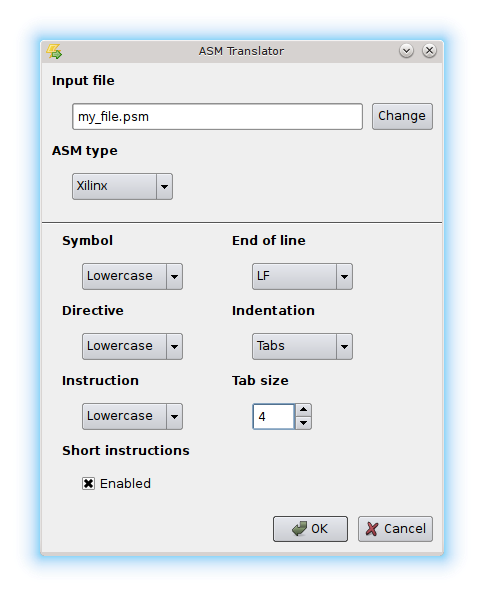
\includegraphics[width=.5\textwidth]{img/ASM_translator.png}
            \caption{ASM translator}
        \end{figure}

    \clearpage
    \subsection{Data file converter}
        This tool allows you to convert selected data file to another. Mutual conversion can be made between .mem, .rawhex, .v, and .vhd, .ihex, .bin, and .srec files.
        \begin{description}
            \item[Section Input File] Here you can select desired input data file which will be converted.
            \item[Section Input Options] In this section, you define what type of input file will be converted.
            \item[Input file type] Available options - Hex, Bin, SRec, XilMem, XilVerilog, and XilVhdl.
            \item[Bytes per record] Only if you want to convert XilMem file. Defines number of bytes per record.
            \item[OPCode size] Defines opcode size of selected data file. Available are 16 and 18.
            \item[Section Output File] Defines target.
            \item[Section Output Options] Here you can select desired output data file.
            \item[Input file type] Available options - Hex, Bin, SRec, XilMem, XilVerilog and XilVhdl.
            \item[Tab size]  Define number of inserted spaces when you press Tab.
            \item[Short instructions] Here you can allow short instructions like LD, RETI, etc.
        \end{description}

        \enlargethispage{6\baselineskip}
        \begin{figure}[h]
            \centering
            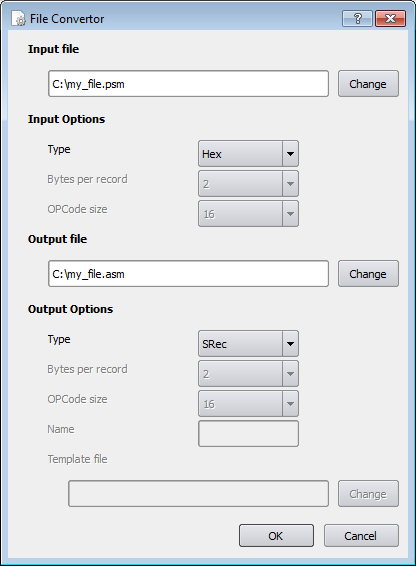
\includegraphics[width=.5\textwidth]{img/DATA_converter.png}
            \caption{DATA file converter}
        \end{figure}

    \clearpage
    \subsection{8-segment editor}
        \begin{wrapfigure}{r}{0pt}
            \centering
            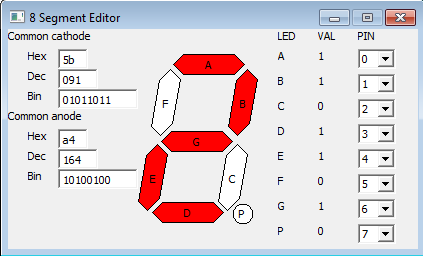
\includegraphics[width=110pt]{img/8segment.png}
            \caption{8-segment editor}
        \end{wrapfigure}
        With this tool you can easily determine what value you have to set on a port to display some digit on numerical LED display. In the left part of the dialog window, you can find numerical values corresponding to the displayed digit. These values are represented for both common cathode and common anode, and in three numerical bases: hexadecimal, decimal, and binary. Buttons on the left side from entry boxes copies value from the adjacent entry box into clipboard. In the right part of the window you can set which port bit is connected to which LED segment, this sets permutation of the resulting values.

    \subsection{LED panel simulator}
        \begin{wrapfigure}{r}{0pt}
            \centering
            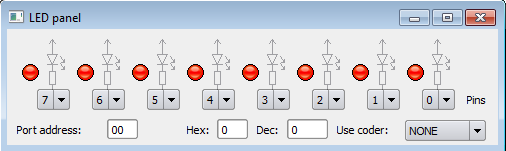
\includegraphics[width=150pt]{img/Led_panel.png}
            \caption{8-segment editor}
        \end{wrapfigure}

        Simple LED panel simulator allows to easily observe output port behavior with visual representation of eight LEDs. You can set BCD and Gray decoder to simulate certain common FPGA logic.

        \begin{description}
            \item[GRAY] Converts output port value to gray code.
            \item[BCD] Output port value will be presented as BCD. Remember that bigger number than 99 cannot be displayed.
        \end{description}

    \subsection{7-segment simulator}
        \begin{wrapfigure}{r}{0pt}
            \centering
            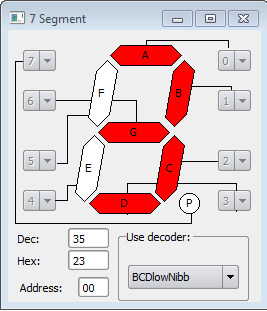
\includegraphics[width=110pt]{img/7seg_sim.png}
            \caption{7-segment simulator}
        \end{wrapfigure}
        Simulator of 7-segment display with common anode, the display is connected to an output port. Port bits can be
        assigned to any display segment. Multiple instances of this simulator can be opened at once. You can set BCD decoder to simulate certain commonly used FPGA logic.

        \begin{description}
            \item[BCDlowNibb] Low-order nibble is decoded and displayed.
            \item[BCDhighNibb] High-order nibble is decoded and displayed.
        \end{description}

    \subsection{Numeric base converter}
        \begin{wrapfigure}{r}{0pt}
            \centering
            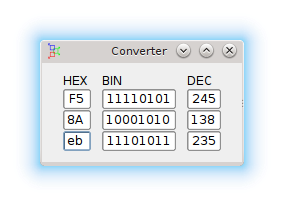
\includegraphics[width=100pt]{img/converter.png}
            \caption{Converter}
        \end{wrapfigure}
        This tool might be useful when you want to quickly convert some number to another radix.
